\section{Methodology}
\label{sec:methodology}

\subsection{Embedding models}
\label{sec:embedding-models}

I undertook this task to investigate the relative performance of pre-trained static and
contextual embeddings for a context-dependent word-similarity task.
The baseline models for the task were the multilingual BERT model
\parencites{Devlin2019} and ELMo models \parencites{Peters2018a} trained on Finnish,
Croatian, and Slovene datasets \parencites{Ulcar2020a},\footnote{I did not directly
  reproduce the baseline models because the first requires the \texttt{bert-embedding}
  Python package, which has been deprecated since 2020 and is incompatible with Apple's
  ARM-based processors \parencites{Lai2023}.
  However, it is notionally equivalent to the contextual embeddings of the
  \texttt{bert-base-multilingual-cased} model with a window size of zero.
} and the vast majority of the task
submissions were based on Transformers \parencites[36,42-45]{Armendariz2020a}, so I
chose to evaluate a variety of pre-trained Transformer models.
Because both static and contextual embeddings can be obtained from a Transformer model,
this approach facilitated a direct comparison between them.
The models that I evaluated were accessed via the HuggingFace \emph{Transformers}
library \parencites{Wolf2020a} and are listed in \cref{table:language-models}.

\begin{table}
  \centering
  \begin{tabular}{lcccc}
    \toprule
    Model name                                                        & English    & Finnish    & Croatian   & Slovene
    \\
    \midrule
    \texttt{EMBEDDIA/crosloengual-bert}\textsuperscript{1}            & \checkmark & \checkmark &
    \checkmark                                                        & \checkmark
    \\
    \texttt{TurkuNLP/bert-base-finnish-cased-v1}\textsuperscript{2}   &            & \checkmark &            &
    \\
    \texttt{TurkuNLP/bert-base-finnish-uncased-v1}\textsuperscript{2} &            & \checkmark &            &
    \\
    \texttt{TurkuNLP/bert-large-finnish-cased-v1}\textsuperscript{2}  &            & \checkmark &            &
    \\
    \texttt{bert-base-cased}                                          & \checkmark &            &            &
    \\
    \texttt{bert-base-multilingual-cased}                             &
    \checkmark                                                        & \checkmark & \checkmark & \checkmark
    \\
    \texttt{bert-base-multilingual-uncased}                           & \checkmark & \checkmark & \checkmark &
    \checkmark
    \\
    \texttt{bert-base-uncased}                                        & \checkmark &            &            &
    \\
    \texttt{bert-large-cased}                                         & \checkmark &            &            &
    \\
    \texttt{bert-large-cased-whole-word-masking}                      & \checkmark &            &            &
    \\
    \texttt{bert-large-uncased}                                       & \checkmark &            &            &
    \\
    \texttt{bert-large-uncased-whole-word-masking}                    & \checkmark &            &            &
    \\
    \texttt{classla-bcms-bertic}\textsuperscript{3}                   &            &            & \checkmark &
    \\
    \bottomrule
  \end{tabular}
  \caption{The pre-trained models from the HuggingFace \emph{Transformers} library
    \parencites{Wolf2020a} that I evaluated for each language.
    The corresponding references are \textsuperscript{1}\textcites{Ulcar2020},
    \textsuperscript{2}\textcites{Virtanen2019},
    \textsuperscript{3}\textcites{Ljubesic2021}, and \textcites{Devlin2019} otherwise.
  }
  \label{table:language-models}
\end{table}

The primary comparison that I made was between the static input and contextual output
representations of these models.
Several of the task submissions used a combination of a Transformer's hidden-states
\parencites[e.g.][276]{Gamallo2020}[61]{CostellaPessutto2020}[145]{Hettiarachchi2020}.
This choice is supported by the analysis of \textcites{Ethayarajh2019}, who found that
the upper layers of Transformer models produce more context-dependent representations.
Hence, I also evaluated an example of pooling hidden-states.
However, a thorough comparison of its variants is beyond the scope of this paper.
\begin{samepage}
  Hereafter, I refer to the kinds of embeddings that I evaluated as:
  \begin{itemize}
    \item \emph{static}, the model's input embeddings;
    \item \emph{contextual}, the model's output embeddings; and
    \item \emph{pooled}, the sum of the model's last four hidden-states.
  \end{itemize}
\end{samepage}

\subsection{Composition operations}
\label{sec:composition-operations}

The basic procedure that I employed is described in \cref{chart:schematic-procedure}.
For each pair of target words and each of the two contexts in which they appear, I
obtained a contextualized representation of a target word by:
\begin{enumerate}
  \item finding the index of the target word's first sub-word token within the tokens of its context;
  \item finding the tokens within a fixed-size window around its first token;
  \item obtaining the embeddings of the tokens in the window; and
  \item composing the embeddings to produce a single representation.
\end{enumerate}
Notably, the use of a sub-word vocabulary by the models in question
\parencites[e.g.][4174]{Devlin2019} dictates that a target word may be represented by a
different number of tokens in each context.
As a result, the similarity between the representations of a pair of target words may
be different in each context, even if the representations are individual static
embeddings.
This is the cause of the non-zero scores obtained by models of this kind, particularly
for the Finnish language (\cref{sec:language-specificity}).

\begin{figure}
  \centering
  \newcommand*{\orawidest}{accept}
  \newcommand*{\oratallest}{\#\#}
  \newlength{\orawidth}
  \settowidth{\orawidth}{\orawidest}
  \newcommand*{\ora}[1]{\overrightarrow{#1\vphantom{\oratallest}}}
  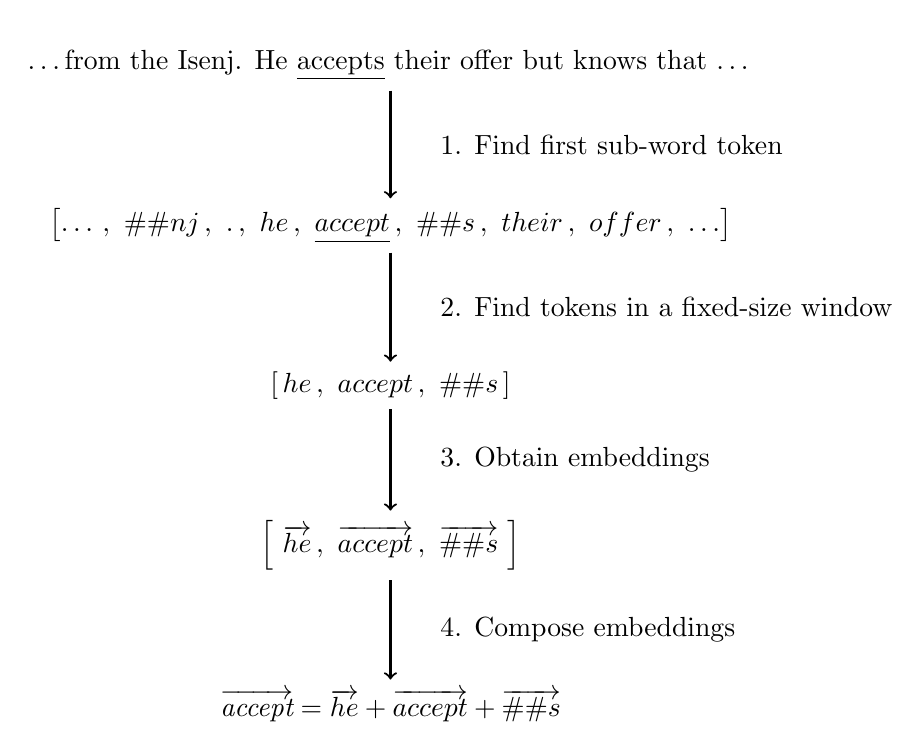
\begin{tikzpicture}[
      every path/.style = {thick, ->},
      every node/.style = {inner sep = 0, outer sep = 0.05in},
      node distance = 0.8in
    ]
    \node [label] (a) {\dots from the Isenj. He \underline{accepts} their offer but knows that \dots };
    \node [label, below of=a] (b) {$\left[ \dots\,,\ \text{\#\#nj}\,,\ .\,,\ \text{he}\,,\ \text{\underline{accept}}\,,\ \text{\#\#s}\,,\ \text{their}\,,\ \text{offer}\,,\ \dots \right]$};
    \node [label, below of=b] (c) {$\left[ \, \text{he}\,,\ \text{accept}\,,\ \text{\#\#s} \, \right]$};
    \node [label, below of=c] (d) {$\left[ \ \ora{\text{he}}\,,\ \ora{\text{accept}}\,,\ \ora{\text{\#\#s}} \ \right]$};
    \node [label, below of=d] (e) {$ \ora{\textit{accept}} = \ora{\text{he}} + \ora{\text{accept}} + \ora{\text{\#\#s}}$};
    \draw (a) -- (b) node[midway, right=0.2in] {1. Find first sub-word token};
    \draw (b) -- (c) node[midway, right=0.2in] {2. Find tokens in a fixed-size window};
    \draw (c) -- (d) node[midway, right=0.2in] {3. Obtain embeddings};
    \draw (d) -- (e) node[midway, right=0.2in] {4. Compose embeddings};
  \end{tikzpicture}
  \caption{A schematic of the procedure used to
    obtain a contextualized representation of a target word from pre-trained embeddings.
    In this example, the target word is ``accept'', the window size is one (either side of
    the target word), and the composition operation is addition.
  }
  \label{chart:schematic-procedure}
\end{figure}

Inspired by \textcites{Landauer1997}, \textcites{Kintsch2001}, and
\textcites{Mitchell2008}, I primarily investigated element-wise addition and
multiplication as composition operations to contextualize embeddings.
The cosine similarity between two vectors is invariant with respect to the
multiplication of the vectors by scalars, so the results of composing the embeddings
within a fixed-size context window by addition or the arithmetic mean are equal.
Hence, I did not investigate the latter.
Preliminary experiments indicated that multiplication performed poorly across all
languages, models, and window sizes, so it was discarded before the final analysis on
the evaluation dataset.
Initially, I also investigated the concatenation (`stacking') of embeddings.
In the case that the number of embeddings was fewer than that expected from the window
size, i.e., the target word was too close to the beginning or end of its context, I
right-padded the concatenated embeddings with zeros to obtain representations of equal
length.
This approach was also generally inferior to addition, as discussed in
\cref{sec:hyperparameter-search}.

\subsection{Window size} \label{sec:window-size}

Due to the computational expense of exhaustively searching the possible window sizes, I
applied heuristics to constrain the search space.
A naïve estimation of the average number of words in each context of the evaluation
dataset, i.e., segmenting on whitespace, gave between $40$ and $60$ for the different
languages.
Therefore, for the static-embedding models, I chose $50$ as an upper bound on the
window size on either side of the target word.
The motivation to choose a smaller maximum window size for contextual-embedding models
was economical, due to their greater computational expense (\cref{sec:cost-benefit}).
However, as the window size approaches the length of the sequence, I expected a
combination of token representations to be superseded by the sequence-level
representation of the model, e.g., the special \texttt{CLS} token of BERT models
\parencites[4174]{Devlin2019}.
These heuristics were largely vindicated by the results on the evaluation dataset,
which showed that the scores decrease as the window size approaches the maximum.
